%-------------------------
% CV Data Engineer - Stephane KPOVIESSI
% Target: Data Engineer / Big Data Engineer / Cloud Data Engineer
%-------------------------

\documentclass[letterpaper,11pt]{article}

\usepackage{latexsym}
\usepackage[empty]{fullpage}
\usepackage{titlesec}
\usepackage[usenames,dvipsnames]{color}
\usepackage{enumitem}
\usepackage[colorlinks=true, urlcolor=primary, linkcolor=primary]{hyperref}
\usepackage{fancyhdr}
\usepackage[french]{babel}
\usepackage{tabularx}
\usepackage{needspace}
\usepackage{graphicx}
\usepackage{tikz}
\input{glyphtounicode}

\definecolor{primary}{RGB}{0, 79, 144}
\definecolor{darkgrey}{RGB}{50, 50, 50}

\usepackage[sfdefault]{noto-sans}
\usepackage[T1]{fontenc}

\pagestyle{fancy}
\fancyhf{}
\fancyfoot{}
\renewcommand{\headrulewidth}{0pt}
\renewcommand{\footrulewidth}{0pt}
\setlength{\footskip}{4.1pt}

\addtolength{\oddsidemargin}{-0.5in}
\addtolength{\evensidemargin}{-0.5in}
\addtolength{\textwidth}{1.0in}
\addtolength{\topmargin}{-0.65in}
\addtolength{\textheight}{1.45in}

\urlstyle{same}
\raggedbottom
\raggedright
\setlength{\tabcolsep}{0in}

\titleformat{\section}{
  \vspace{-4pt}\scshape\raggedright\large\color{primary}
}{}{0em}{}[\color{primary}\titlerule \vspace{0pt}]

\pdfgentounicode=1

\newcommand{\resumeItem}[1]{
  \item\small{{#1 \vspace{-1.5pt}}}
}

\newcommand{\resumeSubheading}[4]{
  \vspace{1pt}\item
    \begin{tabular*}{0.97\textwidth}[t]{l@{\extracolsep{\fill}}r}
      {\color{primary}\textbf{#1}} & #2 \\
      \textit{\small#3} & \textit{\small #4} \\
    \end{tabular*}\vspace{-4pt}
}

\newcommand{\resumeProjectHeading}[2]{
    \Needspace{6\baselineskip}
    \vspace{2pt}\item
    \begin{tabular*}{0.97\textwidth}{l@{\extracolsep{\fill}}r}
      \small#1 & #2 \\
    \end{tabular*}\vspace{-3pt}
}

\renewcommand\labelitemii{$\vcenter{\hbox{\tiny$\bullet$}}$}
\newcommand{\resumeSubHeadingListStart}{\begin{itemize}[leftmargin=0.15in, label={}]}
\newcommand{\resumeSubHeadingListEnd}{\end{itemize}}
\newcommand{\resumeItemListStart}{\begin{itemize}[leftmargin=0.15in, label={\small\textbullet}, itemsep=1.5pt, parsep=0pt, topsep=2pt, partopsep=0pt]}
\newcommand{\resumeItemListEnd}{\end{itemize}\vspace{-1pt}}

\begin{document}

\noindent
\begin{minipage}[c]{0.20\textwidth}
  \centering
  \begin{tikzpicture}
    \begin{scope}
      \clip (0,0) circle (1.45cm);
      \node at (0,0) {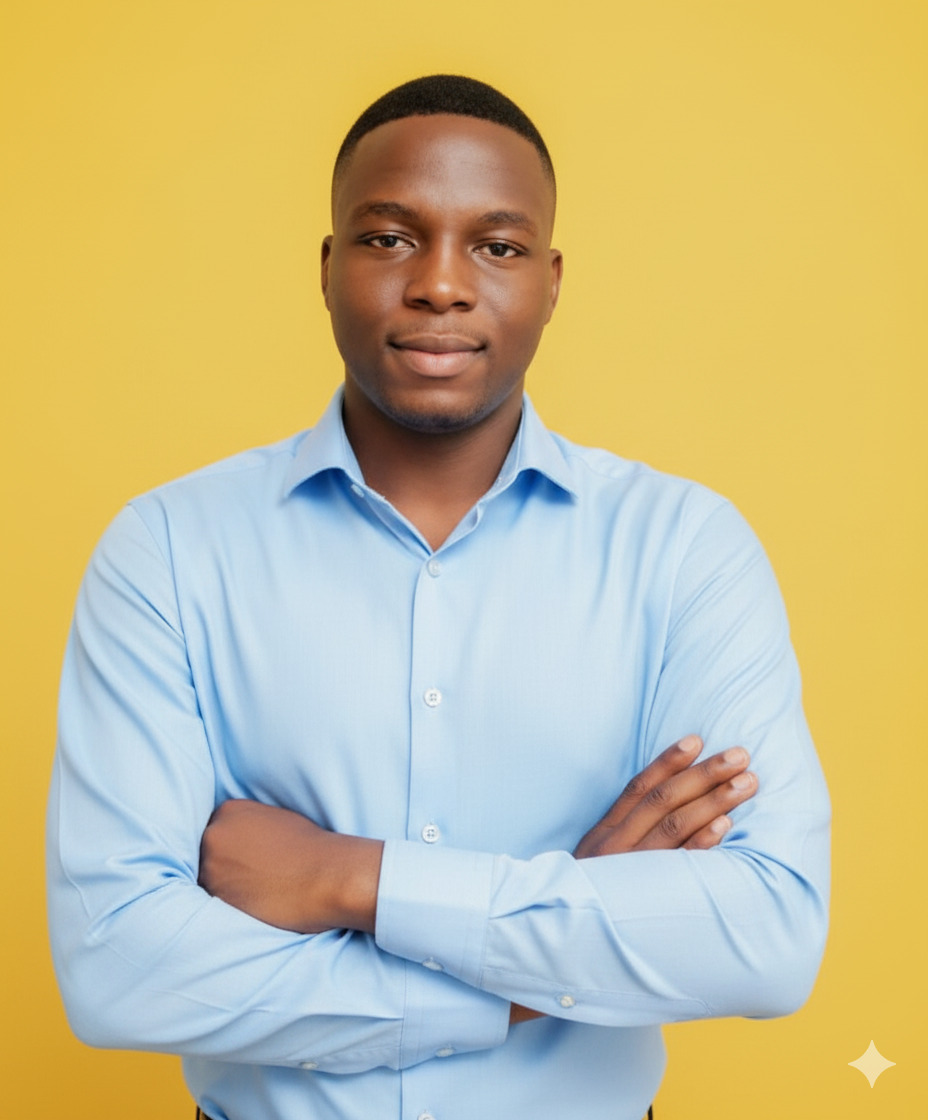
\includegraphics[width=2.9cm]{./profile.jpeg}};
    \end{scope}
    \draw[color=primary, line width=1.2pt] (0,0) circle (1.45cm);
  \end{tikzpicture}
\end{minipage}%
\hspace{0.01\textwidth}%
\begin{minipage}[c]{0.77\textwidth}
  \centering
  {\Huge \scshape \color{primary} Stéphane KPOVIESSI} \\[3pt]
  {\large \textbf{Data Engineer | Python, PySpark \& Azure Databricks}} \\[7pt]
  \small
  Île-de-France (Cergy)
    \enspace$|$\enspace Disponible en CDI
    \enspace$|$\enspace +33\,7\,48\,59\,47\,13 \\[2pt]
  \href{mailto:oastephanekpoviessi@gmail.com}{oastephanekpoviessi@gmail.com}
    \enspace$|$\enspace
  \href{https://linkedin.com/in/stephanekpoviessi}{LinkedIn}
    \enspace$|$\enspace
  \href{https://github.com/EngineerProjects}{GitHub}
    \enspace$|$\enspace
  \href{https://seshat-ai.com}{Seshat-AI}
    \enspace$|$\enspace
  \href{https://kpoviessi-stephane.vercel.app/}{Portfolio}
\end{minipage}
\vspace{3pt}

\section{Profil}
\small{
Ingénieur Big Data \& Data Science orienté \textbf{Data Engineering}, spécialisé dans la conception, la migration et l'industrialisation de pipelines de données fiables. Expérience chez Allianz France sur un projet de migration SAS vers \textbf{Python/PySpark} et \textbf{Azure Databricks}, avec architecture Médaillon, règles métier, data quality et tests de non-régression. Solide socle en SQL, PostgreSQL, ETL/ELT, orchestration, Docker, Git et APIs, complété par une culture Data/IA permettant de construire des plateformes robustes, documentées et exploitables par les équipes métier.
}
\vspace{4pt}

\section{Expériences Professionnelles}
\resumeSubHeadingListStart

\resumeSubheading
{Ingénieur Data / Data Scientist}{Nov. 2025 -- Avr. 2026}
{Allianz France --- Direction P4D, Équipe Advanced Data \& Climate}{Paris, France}
\resumeItemListStart
  \resumeItem{Migration d'un datamart Assurance de SAS vers \textbf{Python/PySpark}, avec validation de la parité fonctionnelle sur plus de \textbf{15 000 lignes de code}.}
  \resumeItem{Implémentation d'une architecture \textbf{Médaillon} sur \textbf{Azure Databricks}, intégrant plus de \textbf{150 règles de gestion métier} pour produire des datasets fiables.}
  \resumeItem{Conception et automatisation d'un pipeline de \textbf{Data Quality géospatiale} pour valider les données, détecter les anomalies et sécuriser les traitements aval.}
  \resumeItem{Développement d'un framework de \textbf{tests automatisés SAS/Python} pour comparer les KPI, contrôler les écarts et sécuriser la non-régression avant production.}
  \resumeItem{Rédaction de documentation technique sur l'architecture, les pipelines, les règles de gestion, les contrôles et les procédures de maintenance.}
\resumeItemListEnd

\resumeSubheading
{Data Analyst -- Missions d'appui stratégique}{2023 -- 2025}
{LYNE ET FRERES SARL \normalfont\small(Missions récurrentes d'analyse Data)}{Ikpinlè, Bénin / À distance}
\resumeItemListStart
  \resumeItem{Structuration et exploitation de données commerciales, opérationnelles et de marché avec \textbf{Python/Pandas} pour suivre les indicateurs clés.}
  \resumeItem{Mise en place de rapports et applications interactives avec \textbf{Streamlit}, HTML/CSS/JavaScript et restitution des analyses aux utilisateurs métier.}
  \resumeItem{Automatisation de traitements récurrents et fiabilisation des données utilisées pour le suivi d'activités agricoles et commerciales.}
  \resumeItem{Accompagnement des utilisateurs dans l'appropriation d'outils data/IA internes et formalisation de recommandations opérationnelles.}
\resumeItemListEnd

\resumeSubheading
{Ingénieur Machine Learning}{Mai 2024 -- Août 2024}
{Groupe Sylvagreg \normalfont\small(Stage)}{Lille, France}
\resumeItemListStart
  \resumeItem{Construction de pipelines de préparation, augmentation et inférence pour une solution de reconstruction 3D à partir d'images 2D.}
  \resumeItem{Industrialisation de traitements Computer Vision sous \textbf{Python/PyTorch}, avec suivi des données d'entrée, sorties et étapes de transformation.}
  \resumeItem{Déploiement cloud sur \textbf{AWS} avec conteneurisation \textbf{Docker} et interface de visualisation pour les utilisateurs métier.}
\resumeItemListEnd

\resumeSubHeadingListEnd

\section{Projets Data Engineering}
\resumeSubHeadingListStart

\resumeProjectHeading
{\textbf{BI Retail Solution} $|$ \emph{Python, PySpark, Airflow, PostgreSQL, Power BI, Docker}}
{\href{https://github.com/EngineerProjects/BI_Retail}{GitHub}}
\resumeItemListStart
  \resumeItem{Mise en place d'une chaîne data de bout en bout : génération et ingestion de données, transformations \textbf{PySpark}, chargement et exploitation analytique.}
  \resumeItem{Modélisation et alimentation d'un \textbf{Data Warehouse PostgreSQL} pour centraliser les données ventes, clients, stocks et supply chain.}
  \resumeItem{Orchestration des traitements avec \textbf{Apache Airflow} et déploiement de l'environnement PostgreSQL/Airflow via \textbf{Docker Compose}.}
  \resumeItem{Production de tableaux de bord Power BI pour valider la valeur métier des datasets : revenus, profits, stocks, pays, magasins et coûts logistiques.}
\resumeItemListEnd

\resumeProjectHeading
{\textbf{Seshat \& Seshat-AI} $|$ \emph{Go, TypeScript, PostgreSQL, RAG, MCP, Multi-Agents}}
{\href{https://github.com/EngineerProjects/seshat}{GitHub}}
\resumeItemListStart
  \resumeItem{Conception d'une plateforme IA modulaire incluant moteur Go, backend local embarqué, backend cloud multi-tenant et application desktop Electron/React.}
  \resumeItem{Développement d'un moteur \textbf{RAG hybride} : ingestion documentaire, chunking, embeddings multi-fournisseurs, recherche vectorielle et orchestration d'agents.}
  \resumeItem{Implémentation de briques orientées production : permissions, auditabilité, gestion de sessions, stockage sécurisé des identifiants et tâches planifiées.}
\resumeItemListEnd

\resumeProjectHeading
{\textbf{Tech Watch Agent} $|$ \emph{Python, FastAPI, LangGraph, PostgreSQL, pgvector, React, Docker}}
{\href{https://github.com/EngineerProjects/tech-watch-agent}{GitHub}}
\resumeItemListStart
  \resumeItem{Développement d'une plateforme de veille automatisée avec collecte multi-source, synthèse structurée, profils récurrents et mémoire sémantique.}
  \resumeItem{Backend \textbf{FastAPI} avec orchestration LangGraph, persistance PostgreSQL/\textbf{pgvector}, configuration de providers LLM/embeddings et stack Docker.}
\resumeItemListEnd

\resumeProjectHeading
{\textbf{Robot autonome de collecte de déchets} $|$ \emph{Python, YOLOv8, OpenCV, Roboflow, Dijkstra}}
{AceObject}
\resumeItemListStart
  \resumeItem{Traitement de données visuelles issues de \textbf{vidéos et images} : extraction, tri, préparation de jeux de données et labellisation avec \textbf{Roboflow}.}
  \resumeItem{Développement d'un pipeline Computer Vision avec \textbf{YOLOv8} et \textbf{OpenCV} pour détecter, classifier et suivre les déchets en les distinguant des obstacles.}
  \resumeItem{Implémentation d'une planification de chemin basée sur \textbf{Dijkstra}, avec exploration du Reinforcement Learning pour la décision autonome et l'évitement d'obstacles.}
\resumeItemListEnd

\resumeSubHeadingListEnd

\section{Compétences}
\begin{itemize}[leftmargin=0.15in, label={}]
\small{\item{
\textbf{Data Engineering} : PySpark, ETL/ELT, Delta Lake, architecture Médaillon, Data Quality, data warehouse, pipelines batch \\
\textbf{Cloud \& Orchestration} : Azure Databricks, Azure Data Lake Storage, Azure Data Factory, AWS, Apache Airflow, Docker, Docker Compose \\
\textbf{Bases de données} : SQL, PostgreSQL, pgvector, modélisation relationnelle, requêtes analytiques, contrôle de cohérence \\
\textbf{Programmation \& APIs} : Python, Pandas, Go, Bash, FastAPI, REST APIs, SSE, tests automatisés \\
\textbf{DevOps \& Industrialisation} : Git, CI/CD, documentation technique, monitoring, reproductibilité, gestion d'environnements \\
\textbf{Data/IA} : Machine Learning, Computer Vision, YOLOv8, OpenCV, Roboflow, RAG, LLMs, embeddings
}}
\end{itemize}

\section{Formation}
\resumeSubHeadingListStart
  \resumeSubheading
    {JUNIA ISEN}{Lille, France}
    {Diplôme d'Ingénieur --- Big Data \& Data Science}{Diplômé en 2026}
  \resumeSubheading
    {JUNIA ISEN}{Rabat, Maroc}
    {Licence --- Électronique et Systèmes Numériques}{2023}
  \resumeSubheading
    {Cycle préparatoire Marie Stella}{Cotonou, Bénin}
    {Classe préparatoire MPSI --- Mathématiques, Physique, Sciences de l'Ingénieur}{2022}
\resumeSubHeadingListEnd

\section{Langues}
\begin{itemize}[leftmargin=0.15in, label={}]
  \small{\item{
   \textbf{Français} : Langue maternelle \vspace{1.5pt} \\
   \textbf{Anglais} : Niveau professionnel (B2 - Certifié Linguaskill Business English) \vspace{1.5pt} \\
   \textbf{Yoruba, Fon, Goun} : Langues maternelles
  }}
\end{itemize}

\section{Engagements \& Associations}
\resumeSubHeadingListStart
  \resumeSubheading
    {Vice-Président}{Sep. 2024 -- Août 2025}
    {Commission Réseau JUNIA ALUMNI}{Lille, France}
    \resumeItemListStart
      \resumeItem{Coordination de la commission, animation du réseau alumni et contribution à l'organisation d'événements professionnels.}
    \resumeItemListEnd

  \resumeSubheading
    {Responsable Communication}{Sep. 2023 -- Août 2024}
    {Commission Réseau JUNIA ALUMNI}{Lille, France}
    \resumeItemListStart
      \resumeItem{Pilotage de la communication, préparation d'annonces et valorisation des initiatives auprès de la communauté.}
    \resumeItemListEnd
\resumeSubHeadingListEnd

\end{document}
